\documentclass[11pt]{article}

\usepackage[margin=1in]{geometry}
\usepackage[T1]{fontenc}
\usepackage[utf8]{inputenc}
\usepackage{lmodern}
\usepackage{microtype}
\usepackage{booktabs}
\usepackage{longtable}
\usepackage{array}
\usepackage{tabularx}
\usepackage{enumitem}
\usepackage{xcolor}
\usepackage{graphicx}
\usepackage{placeins}
\usepackage{hyperref}
\usepackage[numbers,sort&compress]{natbib}

\hypersetup{
  colorlinks=true,
  linkcolor=blue!45!black,
  citecolor=blue!45!black,
  urlcolor=blue!45!black,
  pdftitle={Layered Ashkenazi Jewish Ancestry in One Genome},
  pdfauthor={Daniel S. Goldman}
}

\setlist[itemize]{leftmargin=1.4em}
\setlist[enumerate]{leftmargin=1.6em}
\renewcommand{\arraystretch}{1.15}
\newcolumntype{Y}{>{\raggedright\arraybackslash}X}
\newcommand{\objectheading}[1]{%
  \par\addvspace{0.9\baselineskip}%
  \noindent\textbf{\textit{#1}}\par\nopagebreak\smallskip\noindent%
}

\title{Layered Ashkenazi Jewish Ancestry in One Genome:\\Direct Lineages, Local Haplotype Objects, and Search Targets for Broader Comparison}
\author{Daniel S. Goldman\\\href{https://orcid.org/0000-0003-2835-3521}{ORCID: 0000-0003-2835-3521}}
\date{\today}

\begin{document}
\maketitle

\begin{abstract}
An anonymized Eastern/Central European Ashkenazi Jewish whole genome was compared against public ancient, modern, Jewish, regional, direct-line, family-side, and Roma/Romani data, with controlled or request-bound sources mapped separately. Whole-genome behavior and ROH burden place the genome inside ordinary Ashkenazi variation; the pedigree points into Austro-Hungarian, Hungarian-Slovak, Austrian, Belarusian/Minsk/Stowbtsy, Ukrainian/Kiev, and broader Russian Empire Jewish settings. Broad-source testing makes regional labels meaningful when they resolve into a lineage, local window, carrier set, or concrete data need. Direct-line analysis places the maternal line at \texttt{H1aj1a} and the paternal line at \texttt{R-YP1366*(xR-Y50410)}, downstream of the Ashkenazi-Levite-associated \texttt{R1a-Y2619} lineage. Local autosomal analysis identifies a Lithuanian-supported tract at hg19 chr10:63.8--67.2 Mb, a Jewish/Samaritan/Ashkenazi core at hg19 chr9:71.1--74.2 Mb, and a rare chr3 founder block at hg19 chr3:47.0--49.3 Mb with Mediterranean/eastern-Mediterranean/West-Asian proxy anchors and a structured carrier subclass pattern. A Roma/Romani family story centered on Rebecca/Rivka Reubenstein in the maternal-grandfather branch receives a targeted open-data audit; current open references support an Ashkenazi-centered interpretation and make matched Central/Eastern European Roma references the key test for any smaller branch-level residue. The resulting targets concern Ashkenazi founder structure, Levite-associated paternal lines, northeastern Jewish inheritance, Jewish-region haplotypes, Mediterranean/West-Asian founder texture, and Roma-adjacent family-history testing.
\end{abstract}

\noindent\textbf{Keywords:} Ashkenazi Jewish ancestry; local haplotypes; founder structure; Y chromosome; R1a-Y2619; R-YP1366; H1aj1a; Romani ancestry; public reference data

\section{Introduction}

An anonymized Eastern/Central European Ashkenazi Jewish genome offers a compact profile of recent Jewish genealogy layered with older founder structure. The family record points from recent New York generations back into Austro-Hungarian, Hungarian-Slovak, Austrian, Belarusian/Minsk/Stowbtsy, Ukrainian/Kiev, and broader Russian Empire Jewish settings. The genetic record is Ashkenazi-centered at whole-genome scale, with its sharper information carried by direct lineages and local windows.

Ashkenazi Jewish population history includes bottlenecks, endogamy, founder effects, and older ancestry shared across Jewish, Mediterranean, eastern-Mediterranean, West Asian, and European contexts \citep{carmi2014,xue2017}. Broad regional affinity works as a starting frame. The analysis gives broad signals interpretive weight when they resolve into a Y branch, a maternal line, tract-scale haplotype, carrier set, or comparator gap that can be tested across datasets.

The named targets are concrete. The paternal line falls inside the Ashkenazi-Levite-associated \texttt{R1a-Y2619} lineage and locally downstream at \texttt{R-YP1366*(xR-Y50410)}. The maternal line is \texttt{H1aj1a}. The autosomes preserve a clean Lithuanian-supported chromosome 10 tract, a compact Jewish/Samaritan/Ashkenazi chromosome 9 object, and a rare chromosome 3 founder block with Mediterranean/eastern-Mediterranean/West-Asian proxy anchors. A Roma/Romani family story centered on Rebecca/Rivka Reubenstein creates a targeted comparator problem.

The central comparison set consists of \texttt{R-YP1366}, chr3:47.0--49.3 Mb, chr9:71.1--74.2 Mb, chr10:63.8--67.2 Mb, and a mapped set of Jewish subgroup, Roma/Romani, late southern-Levant Jewish-context, and exact-carrier data needs. These objects connect the genome analyzed here to Ashkenazi Jewish, Jewish diaspora, northeastern Jewish, Levite-associated, Mediterranean/West-Asian founder, and Roma-adjacent family-history questions.

\section{Person, Pedigree, and Research Lens}

The person in question is Eastern/Central European Ashkenazi Jewish, with recent family history in the New York immigrant world and older branch geography pointing into Hungary, Tokaj, Bodrogkeresztur, Presov/Lubotice, Austria, Stowbtsy/Minsk, Kiev/Ukraine, and broader Russian Empire Jewish settings. United States census, naturalization, Social Security, New York vital and municipal records, and a JewishGen Hungary marriage extract give the strongest documentary footing. Tree-only older leads and social-history clues supply geography and hypothesis space.

The pedigree gives local genetic findings a historical map. Austro-Hungarian and Hungarian-Slovak Jewish branches create one recent axis, with Tokaj/Bodrogkeresztur and Presov/Lubotice as prominent place contexts. Former Russian Empire and northeastern Jewish branches create another, especially Stowbtsy/Minsk and Kiev traditions. The Lithuanian, Belorussian, and broader Litvak-facing genetic signals below become population-level search targets with a plausible recent regional setting.

One Roma/Romani family-story lead is centered on Rebecca/Rivka Reubenstein, an ancestor in the maternal-grandfather branch. That story belongs at branch scale. Roma-adjacent stories appear in family histories across Eastern and Central Europe, and genetic testing requires matched Roma/Romani references plus segment-level support.

Read together, the records and genome produce a personal genetic-genealogical account and a set of shared comparison targets. The lineages, local windows, carrier sets, and comparator gaps can be searched in other people, public cohorts, controlled datasets, and future Jewish, Roma/Romani, and eastern-Mediterranean reference panels.

\section{Evidence Base and Claim Types}

The evidence base is organized by claim type. Whole-genome PCA, ADMIXTURE/Q-style behavior, nearest-neighbor behavior, IBS, IBD patterns, and Ashkenazi-control comparisons establish the population frame. Direct mtDNA and Y-DNA calls supply maternal and paternal lineages that can be compared in public trees and project datasets. Local autosomal claims depend on phased haplotypes, parent side, exact-run sharing, IBD spans, marker density, and ChromoPainter-style donor behavior with anchor-removal checks \citep{lawson2012}. Pedigree records supply place, branch, migration context, and family-story leads.

A private maternal AncestryDNA V1 GRCh37.1 array file was compared against the study target's own AncestryDNA array and against phased local-window calls. The array pair supplied mother-child QC, marker-level parent-side anchors, and family-side checks for candidate windows. Its main role in phase 1 was interpretive calibration: supporting maternal-side coherence for the chromosome 10 Lithuanian tract, paternal-side context for the chromosome 9 core, parent-switch limits for chromosome 12, and the split-block reading that closed the earlier chromosome 2 single-haplotype claim.

The public-facing comparative record includes the Allen Ancient DNA Resource v66.p1, Behar-style Jewish references, Bray/GSE23636 Ashkenazi controls, HGDP high-coverage genomes, processed ancient and historical pilots, open Iberian Roma Human Origins data, South Asian and South-Central Asian references, public mtDNA resources, and FamilyTreeDNA Discover Y-tree JSON for the downstream paternal branch. Among processed historical pilots, Roquetes enters the main chromosome 9 interpretation; Islamic Ibiza, Segesta, Amvrakia, Roca Vecchia, Nahal Yarmuth, and northeast Iberian Iron Age rows mainly define calibrated context.

Claims are strongest where broad affinity, phase-aware sharing, parent-side coherence, exact or IBD support, and stable anchor behavior point to the same window. Sparse ancient samples and modern proxy labels supply context; compact tracts carry the comparison work.

\section{Genome-wide Placement and Local-Object Logic}

Genome-wide behavior is Ashkenazi-centered. PCA, ADMIXTURE/Q-style behavior, nearest-neighbor patterns, IBD behavior, and Ashkenazi-control screens all place the genome analyzed here within Ashkenazi Jewish ancestry. Mediterranean, Levantine, Anatolian, North African, Baltic/Litvak, and broader West Asian directions recur as historical texture inside that frame.

The broad-source search is also a finding. Under current public data, wide Jordanian, Moroccan, Anatolian, Sicilian, Baltic, Samaritan, Roma/Romani, and southern-Levant-facing labels settle into founder-history texture unless a named lineage or compact local window carries the signal. ROH burden sits within ordinary Ashkenazi-control range, so the interpretive weight falls on specific local objects inside an ordinary founder-population background.

Within those boundary conditions, the reusable level is a named lineage, a compact window, a carrier set, or a replication trigger.

Three autosomal objects currently carry the strongest evidence. Chromosome 10 is the cleanest regional or genealogy-grade tract, with Lithuanian/Baltic or Litvak-adjacent support. Chromosome 9 is the strongest compact Jewish-region object, shared across Samaritan and Ashkenazi comparators. Chromosome 3 is the most distinctive rare founder block, visible through Mediterranean, eastern-Mediterranean, and West Asian proxy anchors. Figure~\ref{fig:local-object-map} shows how these retained objects differ from lower-tier and contextual windows.

\begin{figure}[htbp]
\centering
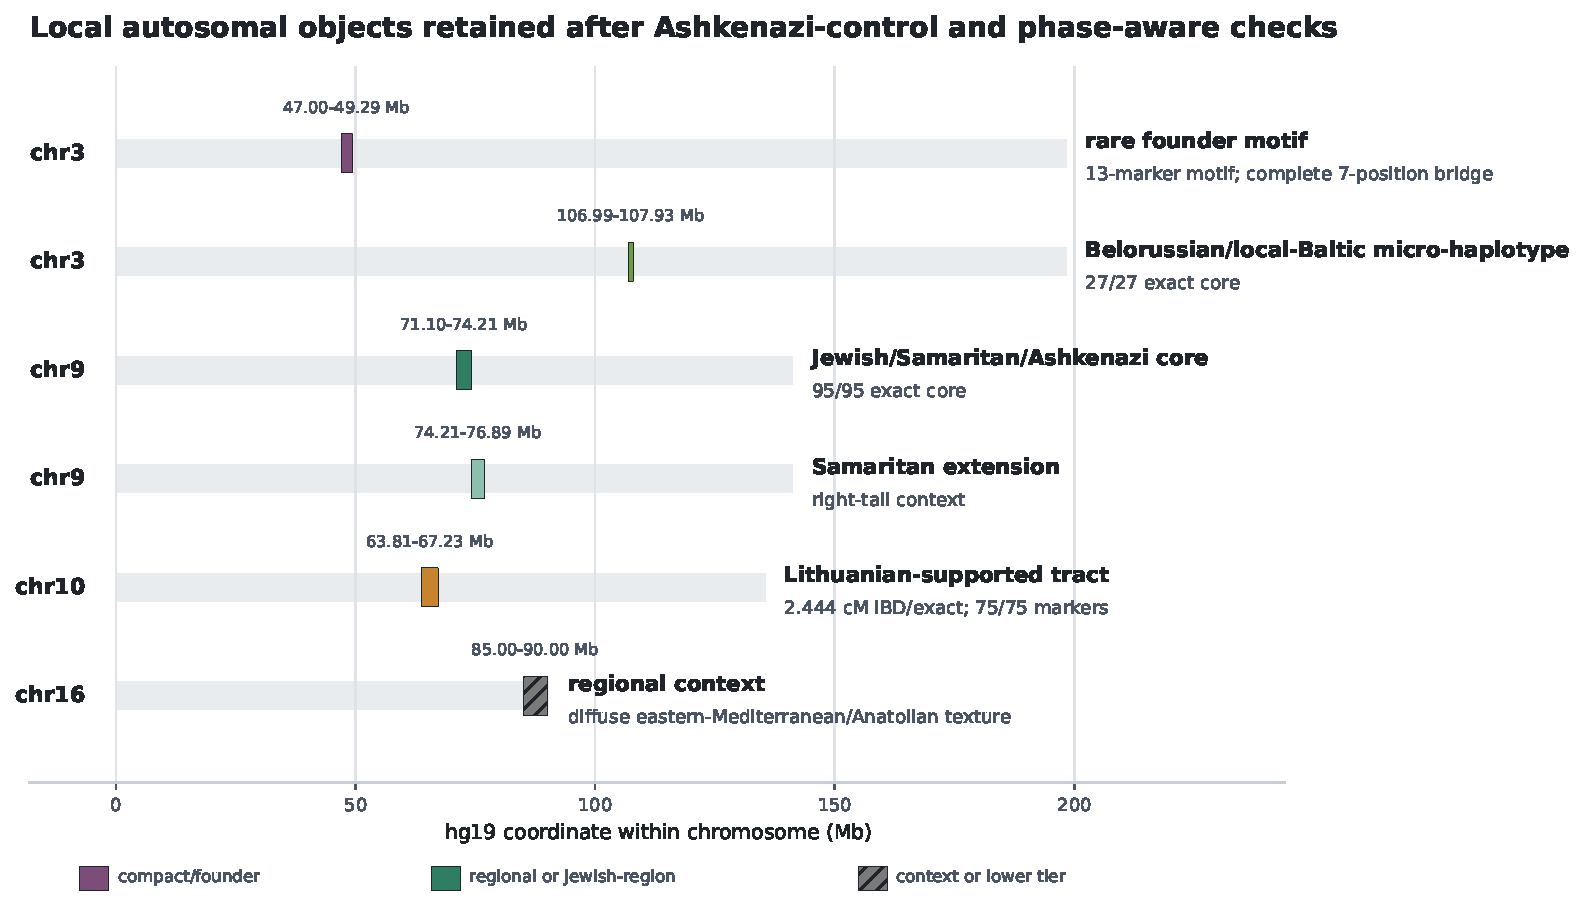
\includegraphics[width=\textwidth]{figures/fig1_local_object_map.pdf}
\caption{Retained local autosomal objects. The map separates high-confidence compact or regional objects from lower-tier and contextual windows, with coordinates shown on their chromosome-specific hg19 axes.}
\label{fig:local-object-map}
\end{figure}
\FloatBarrier

\section{Direct Lineages as Comparison Targets}

The direct maternal line is \texttt{H1aj1a}, supported by HaploGrep quality 0.9535 and strong VCF/BAM evidence. Public context places the line in an Ashkenazi-compatible European and North/Central Mediterranean setting, with Baltic/Litvak-facing echoes in public rows and medieval Jewish Erfurt context \citep{costa2013}. A \texttt{152C}-side context points toward the public uncertain/beta \texttt{H1aj1a1\textasciicircum{}}/\texttt{T152C!} side, with tighter child-marker placement unresolved in current checking. Closest open comparators include Ashkenazi complete mitogenomes and Baltic-facing public rows, making \texttt{H1aj1a} plus the \texttt{152C} context a practical maternal-line search lane.

The direct paternal line is the strongest named lineage target. Y calls place it downstream of the Ashkenazi-Levite-associated \texttt{R1a-Y2619} branch at:

\begin{center}
\small
\texttt{R-YP1366*(xR-Y50410)}.
\end{center}

The path is:

\begin{center}
\small
\texttt{R-Z93} $\rightarrow$ \texttt{R-Z94} $\rightarrow$ \texttt{R-Z2124} $\rightarrow$ \texttt{R-Z2122} $\rightarrow$ \texttt{R-CTS6}\\
$\rightarrow$ \texttt{R-Y2619/FGC10617} $\rightarrow$ \texttt{R-YP1074} $\rightarrow$ \texttt{R-YP1366}.
\end{center}

Current calls place the line separate from the public \texttt{R-Y50410/R-Y50945} side branch. Ten strong private-like Y SNP candidates form a practical comparison packet for future paternal-line matching under or near \texttt{R-YP1366}; \texttt{R-YP1366*(xR-Y50410)} is the public comparison placement.

Rootsi et al. refined the Ashkenazi Levite R1a result through whole-Y sequencing and \texttt{R1a-M582}, finding \texttt{R1a-M582} among all sampled R1a Ashkenazi Levites, among 33.8\% of other sampled R1a Ashkenazi Jewish males, among 5.9\% of sampled R1a Near Eastern males, and absent in 922 sampled Eastern Europeans \citep{rootsi2013}. Behar et al. expanded the whole-Y dataset to 486 Y chromosomes, refined the central Ashkenazi Levite branch as \texttt{R1a-Y2619}, and estimated coalescence at 3,143 years before present for \texttt{R1a-M582} and 1,743 years before present for \texttt{R1a-Y2619} \citep{behar2017}. Their interpretation places \texttt{R1a-Y2619} as an Ashkenazi Levite-associated paternal founder line with Middle Eastern source context and later Ashkenazi expansion.

FamilyTreeDNA Discover estimates for \texttt{R-YP1366} give \texttt{R-Y2619} mean TMRCA 737 CE (range 515--926), \texttt{R-YP1074} 1022 CE (808--1200), \texttt{R-FGC23326} 1129 CE (928--1295), and \texttt{R-YP1366} TMRCA 1406 CE (1252--1531), with \texttt{R-YP1366} formed around 1129 CE. These are source-specific public-tree estimates, complementary to the published whole-Y estimates. Documentary Levite status belongs to family records; the genetic result supplies a concrete downstream branch for matching and tree comparison.

\begin{table}[htbp]
\centering
\caption{Direct-line comparison targets.}
\small
\begin{tabularx}{\textwidth}{p{0.14\textwidth}p{0.23\textwidth}Y Y}
\toprule
Line & Assignment & Population context & Comparison value \\
\midrule
Maternal & \texttt{H1aj1a} & Ashkenazi-compatible European/North-Central Mediterranean line with Baltic/Litvak-facing public context. & Compare against full-sequence mtDNA projects, medieval Jewish context, and Baltic-facing Ashkenazi maternal rows. \\
Paternal & \texttt{R-YP1366*(xR-Y50410)} & Downstream branch of Ashkenazi-Levite-associated \texttt{R1a-Y2619}; public-tree TMRCA centered around 1406 CE. & Search Y projects and public trees for documented Ashkenazi Levite-associated and neighboring non-Levite families. \\
\bottomrule
\end{tabularx}
\end{table}

\section{Local Autosomal Objects as Search Targets}

The autosomal results divide into three main searchable objects. Chromosome 10 is the cleanest genealogy-grade tract for northeastern Jewish and Litvak-adjacent matching. Chromosome 9 is the strongest Jewish-region haplotype object. Chromosome 3 is the strongest rare anthropological signal, a compact founder block that asks for carrier expansion.

\objectheading{Chromosome 10 Lithuanian-supported tract.}
The cleanest regional tract spans hg19 chr10:63,809,527--67,227,685. On haplotype 2, the genome analyzed here shares a 2.444 cM IBD/exact segment with \texttt{lithuania3} haplotype 1, with 75/75 selected-pair markers and maternal-side coherence. ChromoPainter independently recovers \texttt{lithuania3} as the dominant donor in the same interval. The tract fits recent or semi-recent northeastern/Baltic/Litvak-adjacent inheritance inside an Ashkenazi genome and gives a concrete segment for co-segregation, match triangulation, and branch testing.

\objectheading{Chromosome 9 Jewish/Samaritan/Ashkenazi object.}
The chromosome 9 core spans hg19 chr9:71,103,406--74,208,282. The paternal-side haplotype shares a 95/95 exact core with \texttt{Samaritian988} hap2 and \texttt{ashkenazy8w} hap2. \texttt{Samaritian988} extends exact sharing through chr9:76,891,412, matching the local IBD span. In ChromoPainter anchor checks, the signal moves between the Ashkenazi and Samaritan anchors when either is removed, then falls into lower-tier patchwork context when both anchors are removed.

The strongest reading is an older Jewish/Samaritan/Ashkenazi local object preserved inside Ashkenazi founder ancestry. Roquetes medieval Jewish Catalonia data provide broad/core chromosome 9 context, especially in the denser rows processed locally. The natural comparator set includes Jewish, Samaritan, Karaite, Sephardi, Mizrahi, North-African Jewish, and late southern-Levant Jewish-context datasets. A third near-exact carrier, dense Jewish subgroup panel, or direct Jewish-context ancient genome is the strongest upgrade.

\objectheading{Chromosome 3 rare-motif founder block.}
The most distinctive autosomal object spans hg19 chr3:47,002,931--49,291,883. Within this interval, a 13-marker sparse-panel motif was used to compare carriers, with seven of those positions forming the bridge state used for subclassing. The genome analyzed here carries the complete seven-position bridge state \texttt{1111111} on one phased haplotype. The motif links to \texttt{Jordan546}, \texttt{Adana23108.HO}, \texttt{HGDP00635.HO}, \texttt{Y064.HO}, \texttt{moroccoC61}, and \texttt{HGDP00672.HO}. The complete bridge is currently unique in the available phased panel, with external carriers sorting into bridge subclasses around a shared inner/right block: a primary \texttt{0111111} subclass in \texttt{Adana23108.HO}, \texttt{HGDP00635.HO}, \texttt{Y064.HO}, and \texttt{moroccoC61}; an alternate \texttt{1011111} subclass in \texttt{HGDP00672.HO}; and a \texttt{0001111} full-block subclass in \texttt{Jordan546}.

ChromoPainter anchor validation gives the block its weight. In the baseline, the Mediterranean and West Asian focus bucket is high, with \texttt{Jordan546} and \texttt{moroccoC61} as the strongest donors. Removing \texttt{moroccoC61} leaves the signal mainly through \texttt{Jordan546}; removing \texttt{Jordan546} leaves the signal mainly through \texttt{moroccoC61}; removing both collapses the donor-bucket signal. HGDP high-coverage checks identify \texttt{HGDP00635} and \texttt{HGDP00672} as the clearest high-coverage anchors. Figure~\ref{fig:chr3-bridge} gives the bridge subclasses and anchor behavior in one view.

\begin{figure}[htbp]
\centering
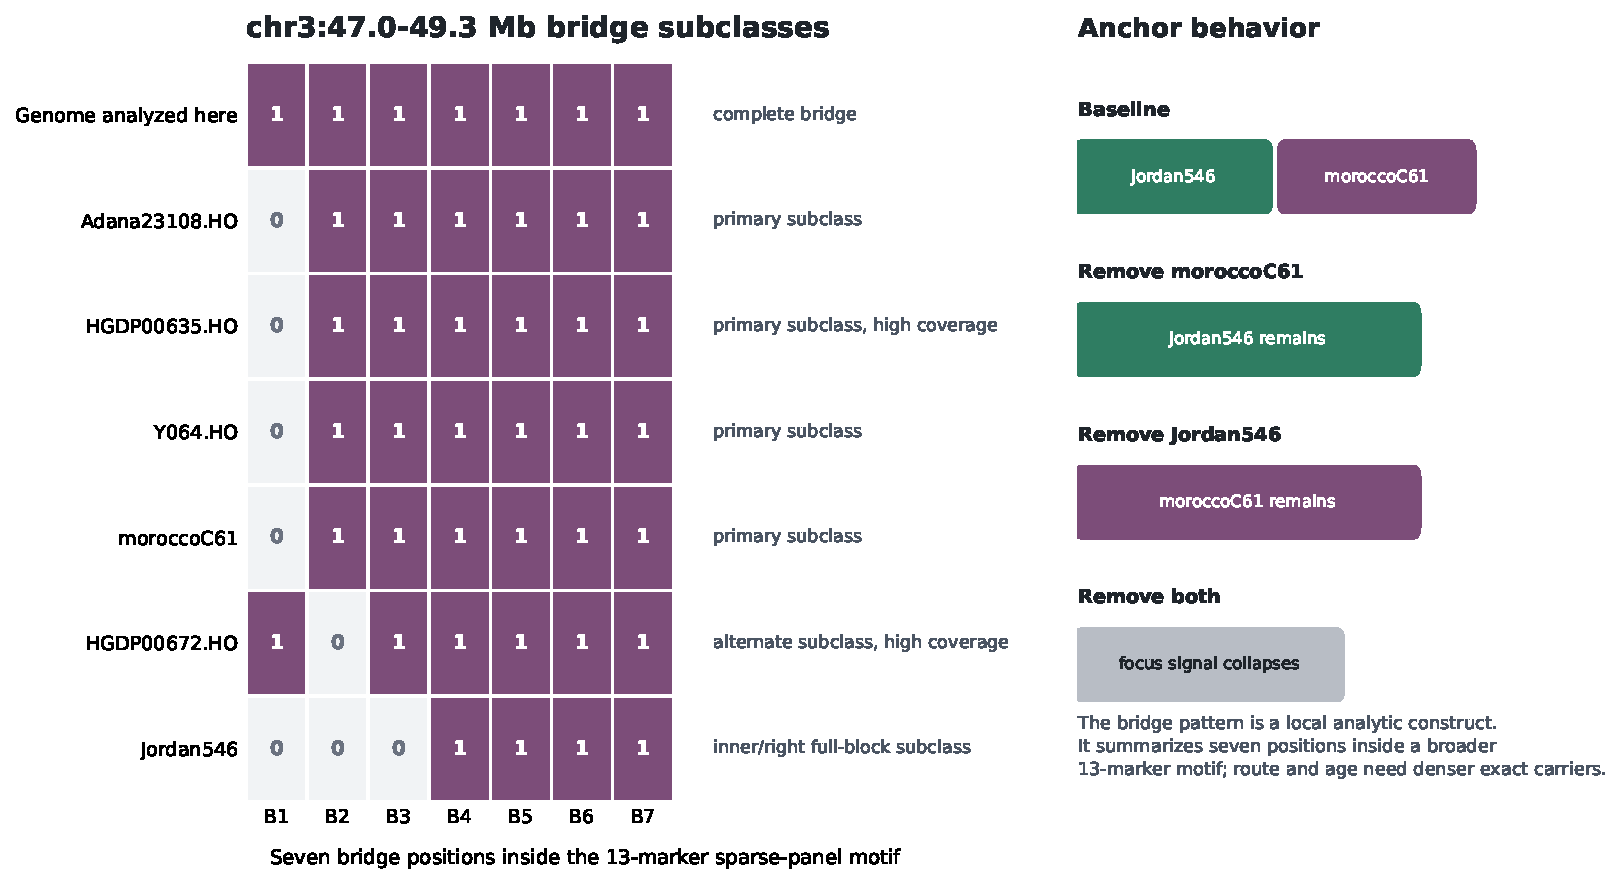
\includegraphics[width=\textwidth]{figures/fig2_chr3_bridge_schematic.pdf}
\caption{Chromosome 3 bridge subclasses and anchor behavior. The bridge summarizes seven positions inside the broader 13-marker sparse-panel motif; the complete bridge appears on the genome analyzed here, and related external carriers sort into partial-bridge subclasses around a shared inner/right block.}
\label{fig:chr3-bridge}
\end{figure}
\FloatBarrier

This is the strongest compact anthropological finding in the genome analyzed here. Current evidence supports a real founder block with Mediterranean, eastern-Mediterranean, and West Asian proxy structure. Dense exact carriers can turn the local observation into a better-dated, better-routed founder object across Jewish diaspora, Mediterranean, eastern-Mediterranean, West Asian, North-African Jewish, and potentially Roma-adjacent panels.

\objectheading{Secondary and context signals.}
The chr3 Belorussian/local-Baltic micro-haplotype at approximately hg19 chr3:106.986--107.926 Mb is credible and lower tier. Haplotype 1 shares a 27/27 exact core with \texttt{belorus5} haplotype 1, with a paternal anchor inside the core. It supplies a second northeastern search point below the chromosome 10 tract.

The chr16:85--90 Mb region is broader regional context. Its texture points toward Anatolian and Byzantine-adjacent, West Asian, eastern-Mediterranean, and Jewish Mediterranean contexts, with diffuse expanded IBD and haplotype behavior. Broad Mediterranean, Italy, Sicily, Punic, Aegean, Anatolian, and Maghrebi axes recur across the work; Ashkenazi controls absorb many broad peaks. These axes remain background until a compact local object emerges.

\begin{table}[htbp]
\centering
\caption{Autosomal search targets and replication triggers.}
\small
\begin{tabularx}{\textwidth}{>{\raggedright\arraybackslash}p{0.24\textwidth}Y Y Y}
\toprule
Object & Key support & Comparison value & Replication trigger \\
\midrule
chr10:63.81--67.23 Mb & 2.444 cM IBD/exact tract; 75/75 markers; maternal-side coherence; \texttt{lithuania3}. & Northeastern Jewish, Baltic, and Litvak-adjacent segment comparison. & Co-segregating matches or denser Baltic/Litvak Jewish references. \\
chr9:71.10--74.21 Mb & 95/95 exact core with \texttt{Samaritian988} and \texttt{ashkenazy8w}; Samaritan extension; anchor switching. & Jewish-region haplotype search across Ashkenazi, Samaritan, Karaite, Sephardi, Mizrahi, and North-African Jewish data. & Third near-exact carrier, Jewish subgroup panel, or late southern-Levant Jewish-context genome. \\
chr3:47.00--49.29 Mb & Seven-marker \texttt{1111111} bridge; 13-marker carrier set; anchor behavior around \texttt{Jordan546} and \texttt{moroccoC61}. & Rare founder-block search across Jewish diaspora, Mediterranean, eastern-Mediterranean, West Asian, and related panels. & Dense exact carriers or sequence-grade data for named carriers. \\
chr3:106.986--107.926 Mb & 27/27 exact core with \texttt{belorus5}; paternal anchor; lower-tier support. & Secondary northeastern/local-Baltic search point. & Threshold IBD or additional exact carriers. \\
\bottomrule
\end{tabularx}
\end{table}

\section{Roma/Romani Family-Story Testing}

The Roma/Romani story is a family-memory lead centered on Rebecca/Rivka Reubenstein, an ancestor in the maternal-grandfather branch. The genetic audit did not localize the question to Rebecca/Rivka or to that branch; it tested whether the genome analyzed here shows segment-real Roma/South-Asian excess under the available open references. The open-data audit used 33 Iberian Roma Human Origins samples, 527 South Asian core references, 258 Iranian/South-Central Asian references, Iberian and South-European baselines, and eight Ashkenazi controls. The panel is adequate for a first audit and geographically indirect for a Central/Eastern European family story.

Whole-genome contrasts are flat. The genome analyzed here has Roma\_Iberian z = -0.020610, SouthAsian\_core z = 0.354954, and IranianPlateau\_SouthCentralAsian z = 0.583976; differential contrasts are also flat, with Roma-minus-Iberian z = -0.057944 and SouthAsian-minus-Iberian z = 0.914234. Differential 10 Mb outlier windows exist, including several z >= 3 rows, and their distribution is scattered; a coherent Roma-plus-South-Asian tract pattern has yet to appear in current data.

Current open references point to an Ashkenazi-centered interpretation. Any Roma/Romani residue is likely tiny, older, socially mediated, or dependent on better matched regional references. Roma-adjacent family stories in Eastern/Central European Jewish pedigrees need matched regional Roma references and segment-level support. The best identified upgrade is EGA \texttt{EGAD50000001103}, a managed-access Human Origins array dataset with 42 Czech Roma and 52 Czech non-Roma samples, much better matched to a Central/Eastern European question than the open Iberian Roma panel alone.

\section{Comparator Map and Replication Targets}

The next comparisons are specific. Modern Jewish subgroup panels are the highest-priority genome-wide comparator gap. Kopelman et al. 2020 is expected to sharpen Sephardi, Mizrahi, North-African Jewish, Balkan/Ottoman Jewish, and finer Jewish regional context around chr9, chr3, and whole-genome texture. Atzmon/Hao/Ostrer 2010 remains a valuable legacy Jewish diaspora panel if derived genotype access becomes available \citep{atzmon2010}. These sources are most relevant for chr9 and chr3, where Jewish subgroup structure may explain signals now visible through broader proxies.

The major ancient-data need is late southern-Levant Jewish-context genome-wide data from Judea, Galilee, Jerusalem, or clearly Jewish southern-Levant settings around roughly 300 BCE--300 CE. Existing adjacent Levantine, Phoenician, Lebanese, Anatolian, Aegean, and Mediterranean proxies frame the question \citep{haber2013}. Direct Jewish-context genomes would sharpen source language across the chr9 and chr3 interpretations.

The chr3 rare motif needs exact-carrier expansion. The priority named carriers are:

\begin{center}
\small
\texttt{Adana23108.HO}, \texttt{Y064.HO}, \texttt{moroccoC61},\\
\texttt{Jordan546}, and additional exact carriers.
\end{center}

HGDP00635 and HGDP00672 already provide high-coverage anchors. The listed full-block carriers remain the limiting layer because several currently appear through sparse or source-limited representations. Dense or sequence-grade data for this set can turn the block from a strong local observation into a carrier-cohort analysis with better age and route inference.

Processed historical pilots sharpen the surrounding map. Roquetes contributes chromosome 9 Jewish-context signal; Islamic Ibiza and Segesta supply broader chr9/chr7 historical texture; Amvrakia, Roca Vecchia, Nahal Yarmuth, and northeast Iberian Iron Age rows remain calibrated context for older Mediterranean, eastern-Mediterranean, and West-Asian-facing comparisons. Figure~\ref{fig:comparator-matrix} condenses the data lanes most likely to sharpen each retained target.

\begin{figure}[htbp]
\centering
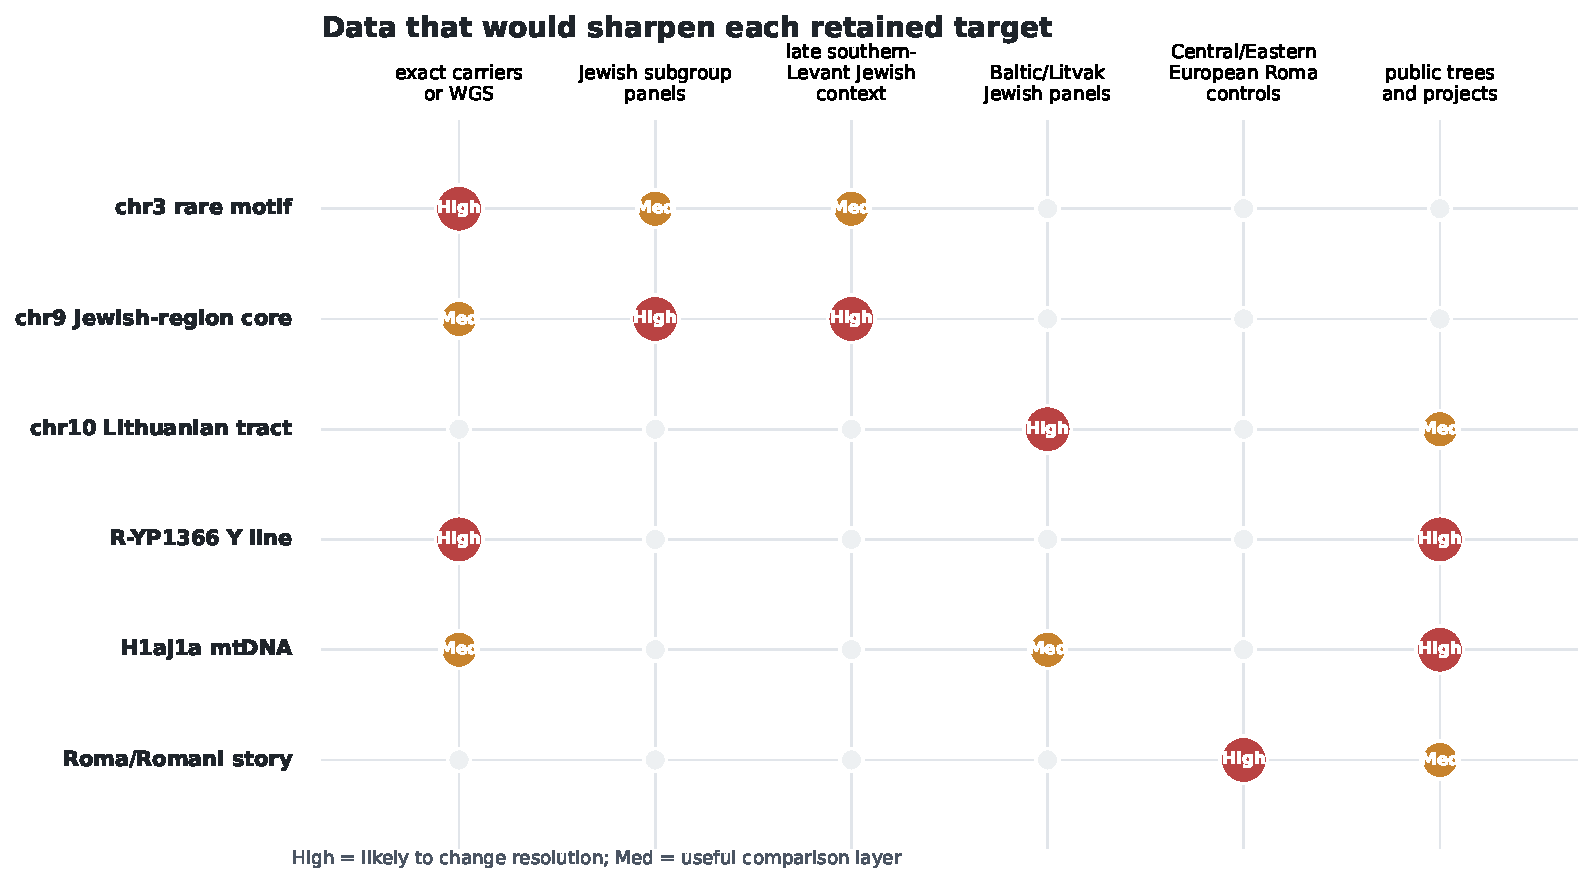
\includegraphics[width=\textwidth]{figures/fig3_comparator_matrix.pdf}
\caption{Data types most likely to sharpen each retained target. High-priority cells mark comparisons likely to change resolution; medium-priority cells mark useful comparison layers.}
\label{fig:comparator-matrix}
\end{figure}
\FloatBarrier

The Roma/Romani family-story question needs matched Central, Eastern, and Balkan European Roma and non-Roma references. The EGA Czech Roma dataset is the clearest identified source. Broader panels from Font-Porterias, Mendizabal, Moorjani, Banfai, and Bianco remain important literature layers, with access routed through controlled, request, or non-direct public paths \citep{font2019,moorjani2013,banfai2018}.

Y-DNA follow-up is a separate route. Public project trees, YFull/FTDNA-style resources, and future matches under \texttt{R-YP1366} or neighboring branches can refine the downstream paternal position relative to documented Ashkenazi Levite-associated and non-Levite families.

\section{Discussion}

The person in question sits within Eastern/Central European Ashkenazi Jewish history, with a recent pedigree spanning Austro-Hungarian/Hungarian-Slovak, Austrian, Belarusian/Minsk/Stowbtsy, Ukrainian/Kiev, and broader Russian Empire Jewish contexts. Genome-wide evidence supplies the Ashkenazi frame. Broad-source closure is part of the result: Mediterranean, Levantine, Anatolian, North-African, Baltic/Litvak, Samaritan, Roma/Romani, and West-Asian-facing labels gain interpretive force here when a lineage, tract, carrier set, or matched comparator supports them. The direct lines and local windows give the broad frame its sharper population-historical content.

The direct lines supply two durable matching targets. \texttt{R-YP1366*(xR-Y50410)} is the strongest direct-line result. It sits inside Ashkenazi-Levite-associated \texttt{R1a-Y2619}, has a public-tree TMRCA centered in the late medieval period, and marks a downstream branch of a major Ashkenazi paternal founder lineage. The ten private-like Y SNP candidates give future matches a specific comparison packet within the public branch. \texttt{H1aj1a} plus the \texttt{152C} context gives the maternal side a comparable search lane across Ashkenazi, Baltic-facing, and North/Central Mediterranean complete-mitogenome data.

The strongest autosomal anthropological object is the chr3 rare motif. It is compact, unusual, bridge-structured, and visible through a striking carrier set anchored by Mediterranean, eastern-Mediterranean, and West Asian proxies. The subclass pattern matters: the genome analyzed here carries the full bridge, while named carriers distribute around related partial bridges and a shared inner/right block. HGDP00635 and HGDP00672 already give high-coverage anchors; the source-limited full-block carriers are the key route into age, route, and community-setting inference.

The chr9 object is the strongest Jewish-region haplotype target. Its paternal-side core shared with Samaritan and Ashkenazi comparators, plus Roquetes medieval Jewish Catalonia context, creates a concrete window for Jewish, Samaritan, Karaite, Sephardi, Mizrahi, North-African Jewish, and direct southern-Levant Jewish-context data. The chr10 Lithuanian-supported tract is the best genealogy-grade segment and the clearest local northeastern/Litvak-adjacent signal.

The secondary windows add texture around the main interpretation. The chr3 Belorussian micro-haplotype adds a lower-tier northeastern search point below the chromosome 10 tract. The chr16 regional signal sketches an eastern-Mediterranean and Anatolian-facing edge already common in broader Ashkenazi-founder context, awaiting a tighter local object before it carries heavier interpretive weight.

While the maternal AncestryDNA array yields more limited data than WGS, it can still provide useful information about this lineage at personal and broader comparative scales. In phase 2, it can be studied directly as a SNP-array profile for the mother and as a parent-side anchor for the study target: standalone array placement, broader parent-informative annotation, maternal-versus-paternal summaries across retained and paused windows, and checks against the WGS/phased local objects. The full use of the admittedly less dense maternal AncestryDNA array may still therefore separate direct maternal-line mtDNA from maternal-side autosomal inheritance, paternal-required alleles, and unresolved intervals.

The Roma/Romani family story becomes a bounded comparator problem. The pedigree preserves a real branch-level story, and current open-reference genetics supports an Ashkenazi-centered interpretation. Any Roma/Romani residue appears likely to be tiny, older, socially mediated, or dependent on matched regional references. Central/Eastern European Roma and non-Roma references are the right future test.

The ranked search targets are \texttt{R-YP1366} under Ashkenazi-Levite-associated \texttt{R1a-Y2619}; chr3:47.0--49.3 Mb; chr9:71.1--74.2 Mb; chr10:63.8--67.2 Mb; modern Jewish subgroup panels; late southern-Levant Jewish-context genomes; exact chr3 carriers; and matched Central/Eastern European Roma datasets. Together, these targets bear on Ashkenazi founder structure, Jewish-region haplotypes, northeastern Jewish inheritance, and the genetic testing of Roma-adjacent family stories.

\section{Conclusion}

The person in question comes into focus as an Eastern/Central European Ashkenazi Jew whose genome carries both recent family geography and older founder history. The recent map is concrete: New York immigrant generations lead back toward Hungarian, Slovak, Austrian, Belarusian, Ukrainian, and broader Russian Empire Jewish settings. The genetic center is Ashkenazi, with northeastern Jewish texture, an Ashkenazi-Levite-associated paternal branch, and a maternal line that fits an Ashkenazi-compatible European and North/Central Mediterranean setting with Baltic-facing public echoes.

The strongest reading is Ashkenazi-centered and locally structured. Recent Eastern and Central European Jewish genealogy, an Ashkenazi-Levite-associated paternal branch, a textured maternal line, and several compact autosomal windows occupy different layers of the same profile. The broad label remains the frame; the local objects give that frame its research value.

Broad Mediterranean, Levantine, Anatolian, North-African, Roma/Romani, Samaritan, Baltic, and West-Asian-facing labels stay at the level of founder-history context until they are carried by one of those objects. Similar Ashkenazi-centered genomes gain clearer comparison value when broad regional texture appears as a tract, lineage, or carrier set that can be searched in other families and datasets.

The Roma/Romani family story remains part of the genealogy because it is centered on Rebecca/Rivka Reubenstein and a real family memory. Current open comparisons keep the genetic reading Ashkenazi-centered. Any Roma/Romani residue is likely tiny, older, socially mediated, or dependent on closely matched Central/Eastern European Roma reference panels. The story becomes a named-lead comparator problem, best approached with regional Roma controls and segment-level evidence.

The northeastern and Jewish-region objects add two different kinds of structure. The Lithuanian-supported tract is the cleanest regional inheritance signal and may help triangulate Litvak or Baltic-adjacent branches. The chromosome 9 window is more historical, with a paternal-side Jewish-region segment shared across Samaritan and Ashkenazi comparators and reinforced by medieval Jewish Catalonia context. Together they describe a genome shaped by recent Eastern/Central European Jewish family history and older Jewish-region continuity.

The rare chromosome 3 motif is the most interesting anthropological finding. It is compact, bridge-structured, and carried here in the fullest form currently visible in the available phased panel. Its proxy anchors sit in Mediterranean, eastern-Mediterranean, and West Asian space; its support strengthens because those anchors behave as a coherent local object under anchor-removal checks. The signal has a shape, a carrier set, and a place in the genome.

That makes the chromosome 3 motif the most promising clue for population-level discovery. It may represent older founder texture preserved inside Ashkenazi ancestry: a small inherited block that survived the compression of diaspora history and now appears through scattered carriers and proxy anchors. Its age, route, and community setting remain open, which is exactly why it matters. The most interesting result is also the most open: a compact inherited block, quiet at genome-wide scale, that may preserve one of the older paths by which Ashkenazi founder ancestry gathered its Mediterranean and West Asian texture.

\section*{Data Availability}

A public verification package for this paper is available at \url{https://github.com/dgoldman0/homeless/tree/main/geneticprofile/phase1}. The package includes the paper, figures, canonical hg19 window definitions, claim-to-evidence index, public-safe derived tables, source-run provenance, public dataset/accession inventory, analysis guardrails, and reproducibility notes. Raw genotype, sequencing, phased haplotype, private match, living-person, account-gated, and third-party reference files remain outside the public package. Full target-genome reruns require authorized private inputs; public-reference pilots can be repeated from the listed accessions where source terms allow download and local processing.

\begin{thebibliography}{99}

\bibitem{carmi2014}
Carmi, S. et al. Sequencing an Ashkenazi reference panel supports population-targeted personal genomics and illuminates Jewish and European origins. \emph{Nature Communications} 5, 4835 (2014). \url{https://doi.org/10.1038/ncomms5835}.

\bibitem{xue2017}
Xue, J., Lencz, T., Darvasi, A., Pe'er, I. and Carmi, S. The time and place of European admixture in Ashkenazi Jewish history. \emph{PLoS Genetics} 13, e1006644 (2017). \url{https://doi.org/10.1371/journal.pgen.1006644}.

\bibitem{costa2013}
Costa, M. D. et al. A substantial prehistoric European ancestry amongst Ashkenazi maternal lineages. \emph{Nature Communications} 4, 2543 (2013). \url{https://doi.org/10.1038/ncomms3543}.

\bibitem{rootsi2013}
Rootsi, S. et al. Phylogenetic applications of whole Y-chromosome sequences and the Near Eastern origin of Ashkenazi Levites. \emph{Nature Communications} 4, 2928 (2013). \url{https://doi.org/10.1038/ncomms3928}.

\bibitem{behar2017}
Behar, D. M. et al. The genetic variation in the R1a clade among the Ashkenazi Levites' Y chromosome. \emph{Scientific Reports} 7, 14969 (2017). \url{https://doi.org/10.1038/s41598-017-14761-7}.

\bibitem{haber2013}
Haber, M. et al. Genome-wide diversity in the Levant reveals recent structuring by culture. \emph{PLoS Genetics} 9, e1003316 (2013). \url{https://doi.org/10.1371/journal.pgen.1003316}.

\bibitem{atzmon2010}
Atzmon, G. et al. Abraham's children in the genome era: major Jewish diaspora populations comprise distinct genetic clusters with shared Middle Eastern ancestry. \emph{American Journal of Human Genetics} 86, 850--859 (2010). \url{https://doi.org/10.1016/j.ajhg.2010.04.015}.

\bibitem{lawson2012}
Lawson, D. J., Hellenthal, G., Myers, S. and Falush, D. Inference of population structure using dense haplotype data. \emph{PLoS Genetics} 8, e1002453 (2012). \url{https://doi.org/10.1371/journal.pgen.1002453}.

\bibitem{patterson2006}
Patterson, N., Price, A. L. and Reich, D. Population structure and eigenanalysis. \emph{PLoS Genetics} 2, e190 (2006). \url{https://doi.org/10.1371/journal.pgen.0020190}.

\bibitem{font2019}
Font-Porterias, N. et al. European Roma groups show complex West Eurasian admixture footprints and a common South Asian genetic origin. \emph{PLoS Genetics} 15, e1008417 (2019). \url{https://doi.org/10.1371/journal.pgen.1008417}.

\bibitem{banfai2018}
Banfai, Z. et al. Revealing the impact of the Caucasus region on the genetic legacy of Romani people from genome-wide data. \emph{PLoS ONE} 13, e0202890 (2018). \url{https://doi.org/10.1371/journal.pone.0202890}.

\bibitem{moorjani2013}
Moorjani, P. et al. Reconstructing Roma history from genome-wide data. \emph{PLoS ONE} 8, e58633 (2013). \url{https://doi.org/10.1371/journal.pone.0058633}.

\bibitem{geva2020}
Albers, P. K. and McVean, G. Dating genomic variants and shared ancestry in population-scale sequencing data. \emph{PLoS Biology} 18, e3000586 (2020). \url{https://doi.org/10.1371/journal.pbio.3000586}.

\end{thebibliography}

\end{document}
